\documentclass[12pt, a4paper]{article}

\usepackage[margin=2.5cm]{geometry}
\usepackage[T1]{fontenc}
\usepackage{graphicx}
\usepackage{amssymb}
\usepackage{amsmath}
\usepackage{color}
\usepackage{booktabs}
\usepackage{pgfplots}
\usepackage{multirow}
\usepackage{engord}
\usepackage{soul}
\usepackage{textcomp}
\usepackage{parskip}
\usepackage{setspace}
\usepackage{titlesec}
\usepackage{fancyhdr}
\usepackage{float}
\usepackage{subcaption}
\usepackage{tikz}
\usetikzlibrary{positioning, shapes.geometric}
\pagestyle{fancy}
\usepackage[UKenglish]{babel}
\usepackage[UKenglish]{isodate}
\usepackage[skip=2pt,font=footnotesize,justification=centering]{caption}
\usepackage{natbib}
\usepackage[colorlinks=true, 
    linkcolor=blue,
    citecolor=blue,
    filecolor=blue,
    urlcolor=blue]{hyperref}

\newcommand{\ie}{\emph{i.e.}\ }
\newcommand{\eg}{\emph{e.g.}\ }
\newcommand{\etal}{\emph{et al}}

\lhead{}
\chead{}
\rhead{}
\lfoot{}
\cfoot{\thepage{}}
\rfoot{}
\renewcommand{\headrulewidth}{0pt}
\renewcommand{\footrulewidth}{0pt}

\begin{document}

\onehalfspacing

Date: \today{}     \hfill{} Project supervisors: \\
Word count: 1469  \hfill{} Dr. Aidas Masiliūnas and Dr. Laura Galdikienė 

{\LARGE Endogenous Institutional Choice in Public Goods Games: A Voting Experiment}

{\large Aidas Kriščiūnas, Domantas Venclavičius, Karolis Boguška, Mykolas Baškys}

{\small Vilnius University, Faculty of Economics and Business Administration}

\vspace{0.4in}

\singlespacing
\tableofcontents
\onehalfspacing

\section{Abstract}
This study investigates how groups endogenously choose governance institutions to solve social dilemmas in public goods games. Using a novel experimental design, we examine voting behavior and cooperation patterns across 25 rounds where participants repeatedly select among five institutional mechanisms. The experiment begins with 5 rounds of standard public goods game, followed by 20 rounds where groups vote every 5 rounds to implement institutions including punishment and reward options. Our systematic comparison examines individual vs. collective and punishment vs. reward mechanisms within a 2×2 framework. We test hypotheses regarding institutional preferences, path dependence, and efficiency consequences of different institutional choices. A pilot experiment will test the design structure and participant comprehension.

\section{Introduction}

This experiment examines a fundamental question in experimental economics: how do groups endogenously choose governance institutions to solve social dilemmas, and what are the behavioral and efficiency consequences of these choices? While extensive research has studied the effects of externally imposed institutions on cooperation, much less is known about how groups select their own governance mechanisms through democratic processes.

The classic public goods game demonstrates the tension between individual and collective interests, typically showing a decay in cooperation over time as free-riding behavior dominates \citep{fehr2000}. Previous research has established that institutions like punishment \citep{fehr2000}, rewards \citep{sefton2007}, and collective mechanisms \citep{tao2016} can sustain cooperation when externally imposed. However, the process by which groups choose among these institutions remains underexplored.

\subsection{Research Questions}
\begin{itemize}
    \item Which institutional mechanisms do groups prefer when given multiple options?
    \item How do individual vs. collective institutions affect cooperation?
    \item What are the efficiency consequences of different institutional choices?
    \item Do groups show path dependence in institutional selection?
\end{itemize}

\subsection{Research Gap and Novelty}
Most studies examine single institutions or multiple imposed institutions; we compare multiple endogenously implemented institutional types. Our research provides systematic comparison of individual vs. collective and punishment vs. reward mechanisms within a unified experimental framework.

\section{Literature Review}

The study of institutional solutions to social dilemmas has a rich history in experimental economics. The standard public goods game, developed by \citet{isaac1988}, reliably demonstrates the cooperation decay phenomenon where contributions decrease over repeated rounds despite the social optimum requiring full cooperation.

Research on institutional interventions has shown that punishment mechanisms can sustain cooperation \citep{fehr2000}, though they may reduce overall efficiency due to the costs of punishment. Reward systems have also proven effective, though potentially less efficient than punishment \citep{tao2016}.

\subsection{Theoretical Framework}
Our study builds on several key theoretical perspectives:
\begin{itemize}
    \item \textbf{Behavioral Game Theory}: Considers how psychological factors affect strategic decision-making
    \item \textbf{Social Preference Models}: Incorporates fairness, reciprocity, and inequality aversion
    \item \textbf{Path Dependence Theory}: Suggests that initial institutional choices constrain future options
\end{itemize}

%The concept of endogenous institutional choice represents a significant advancement beyond studying externally imposed rules. \citet{ostrom1990} emphasized that successful common-pool resource management often involves users developing their own governance rules, suggesting that the process of institutional selection may itself affect cooperation outcomes.

\section{Predictions and Hypotheses}

\subsection{Theoretical Predictions}
\begin{itemize}
    \item \textbf{Institutional Preferences}: Groups prefer individual control over automatic systems initially, but may shift toward collective mechanisms as they learn about relative efficiency
    \item \textbf{Punishment vs. Reward}: Punishment favored initially due to salience of free-riding
    \item \textbf{Status Quo Bias}: Groups tend to retain institutions that appear successful
    \item \textbf{Efficiency Trade-offs}: Automatic systems avoid costly sanctioning
\end{itemize}

\subsection{Hypotheses}
\begin{itemize}
    \item \textbf{H1}: Individual punishment will be most popular initially among institutional options
    \item \textbf{H2}: Collective institutions will yield highest efficiency in the long run
    \item \textbf{H3}: Groups will show path dependence in institutional choice (retention rates > 60\%)
    \item \textbf{H4}: Voting patterns will reflect learning from institutional performance
\end{itemize}

\section{Methodology}

\subsection{Experimental Design}
We employ a within-subjects design with 25 total rounds conducted using oTree software. Each group consists of 5 participants (24 groups in main study, 120 total participants), with group composition remaining stable throughout the experiment.

\begin{equation}
\text{Earnings}_i = \text{Endowment} - \text{Contribution}_i + \text{MPCR} \times \sum_{j=1}^{N} \text{Contribution}_j
\end{equation}

where MPCR = 0.4, Endowment = 10 points per round, and N = 5 participants per group.

\subsection{Experimental Procedure}
The experiment proceeds in two main phases:

\begin{figure}[H]
\centering
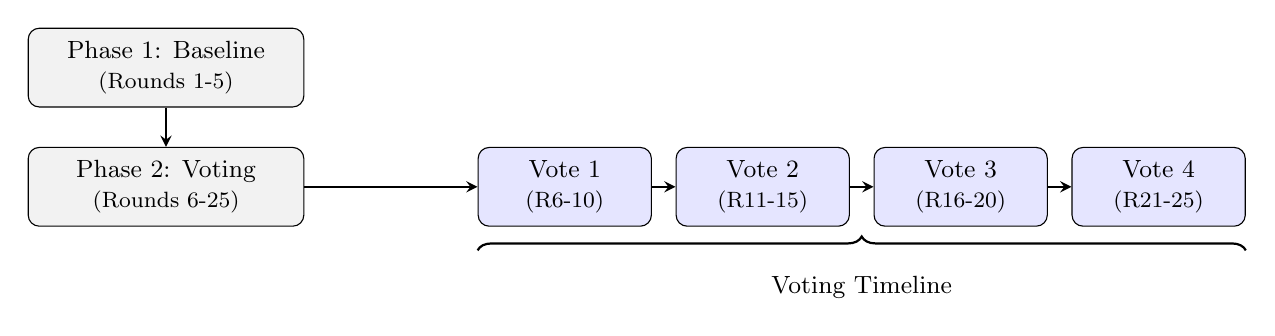
\begin{tikzpicture}[
    node distance=0.3cm,
    box/.style={
        draw, 
        rectangle, 
        rounded corners=4pt,
        minimum width=2.2cm,
        minimum height=1cm,
        align=center,
        font=\small
    },
    phasebox/.style={
        box,
        minimum width=3.5cm,
        fill=gray!10
    },
    votebox/.style={
        box,
        fill=blue!10
    },
    arrow/.style={->, >=stealth, thick}
]

% Main phases - stacked vertically
\node[phasebox] (phase1) {Phase 1: Baseline \\ \footnotesize(Rounds 1-5)};
\node[phasebox, below=0.5cm of phase1] (phase2) {Phase 2: Voting \\ \footnotesize(Rounds 6-25)};

% Voting boxes - in a row
\node[votebox, right=2.2cm of phase2] (vote1) {Vote 1 \\ \footnotesize(R6-10)};
\node[votebox, right=0.3cm of vote1] (vote2) {Vote 2 \\ \footnotesize(R11-15)};
\node[votebox, right=0.3cm of vote2] (vote3) {Vote 3 \\ \footnotesize(R16-20)};
\node[votebox, right=0.3cm of vote3] (vote4) {Vote 4 \\ \footnotesize(R21-25)};

% Main flow arrows
\draw[arrow] (phase1) -- (phase2);
\draw[arrow] (phase2.east) -- (vote1.west);

% Connect voting boxes with arrows
\draw[arrow] (vote1.east) -- (vote2.west);
\draw[arrow] (vote2.east) -- (vote3.west);
\draw[arrow] (vote3.east) -- (vote4.west);

% Optional: Add a bracket/brace to show it's a timeline
\draw[decorate, decoration={brace, amplitude=5pt}, thick] 
    ([yshift=-0.3cm]vote1.south west) -- 
    ([yshift=-0.3cm]vote4.south east)
    node[midway, below=0.2cm] {\small Voting Timeline};

\end{tikzpicture}
\caption{Experimental Timeline with Voting Periods}
\label{fig:experiment-timeline}
\end{figure}

\subsection{Institutional Options}
Participants select from five institutional options every 5 rounds:

\begin{table}[H]
\centering
\caption{2×2 Institutional Framework}
\begin{tabular}{lcc}
\toprule
 & \textbf{Punishment} & \textbf{Reward} \\
\midrule
\textbf{Individual} & Individual Punishment & Individual Reward \\
\textbf{Collective} & Collective Tax & Collective Bonus \\
\bottomrule
\end{tabular}
\end{table}

\begin{enumerate}
\item \textbf{No Institution}: Standard public goods game (baseline)
\item \textbf{Individual Punishment}: Players can punish free-riders at personal cost \citep{fehr2000}
\item \textbf{Collective Tax}: Automatic 20\% tax on uncontributed endowment
\item \textbf{Individual Reward}: Players can reward cooperators at personal cost \citep{sefton2007}
\item \textbf{Collective Bonus}: Automatic rewards for top contributors \citep{tao2016}
\end{enumerate}

\subsection{Mathematical Representation of Institutions}

\textbf{Important design feature:} All institutions maintain identical total endowment (10 points per player per round). Punishment and reward points are deducted from participants' own earnings; no institution provides additional spending capacity that would create endowment disparities.
\begin{itemize}
\item \textbf{Individual Punishment}: 
\begin{equation}
\pi_i = e - c_i + m \sum_{j=1}^{N} c_j - \sum_{j \neq i} p_{ij} - 2\sum_{j \neq i} p_{ji}
\end{equation}
where $p_{ij}$ is punishment points assigned by $i$ to $j$.

\item \textbf{Collective Tax}:
\begin{equation}
\pi_i = 0.8(e - c_i) + c_i + m \sum_{j=1}^{N} c_j
\end{equation}
where 20\% of uncontribued endowment is taxed.

\item \textbf{Individual Reward}:
\begin{equation}
\pi_i = e - c_i + m \sum_{j=1}^{N} c_j + 2\sum_{j \neq i} r_{ji} - \sum_{j \neq i} r_{ij}
\end{equation}
where $r_{ij}$ is reward points assigned by $i$ to $j$.

\item \textbf{Collective Bonus}:
\begin{equation}
\pi_i = 0.8e - c_i + m \sum_{j=1}^{N} c_j + B_i
\end{equation}
where $B_i$ is bonus from pool distributed to top 2 contributors.\footnote{If all contributions are equal, the bonus gets divided equally between all participants.}
\end{itemize}


\subsection{Sample Size and Power Analysis}

Based on established experimental economics standards and power calculations:

\begin{equation}
n = \frac{(Z_{\alpha/2} + Z_{\beta})^2 \times 2\sigma^2}{\delta^2}
\end{equation}

where:
\begin{itemize}
\item $\alpha = 0.05$, $\beta = 0.20$ (power = 80\%)
\item $\sigma$ = expected standard deviation based on previous studies
\item $\delta$ = minimum detectable effect size (medium: 0.5)
\end{itemize}

For our main study: 120 participants (24 groups of 5) provides adequate power for detecting medium effect sizes in within-group comparisons.

\subsection{Data Collection}
We will collect:
\begin{itemize}
\item Contribution decisions (0-10 points each round)
\item Voting choices (4 voting periods)
\item Punishment/reward allocations when applicable
\item Earnings data
\item Demographic information and post-experiment questionnaires
\end{itemize}

\section{Expected Results and Analysis Strategy}

\subsection{Expected Contribution Patterns}

\begin{figure}[H]
\centering
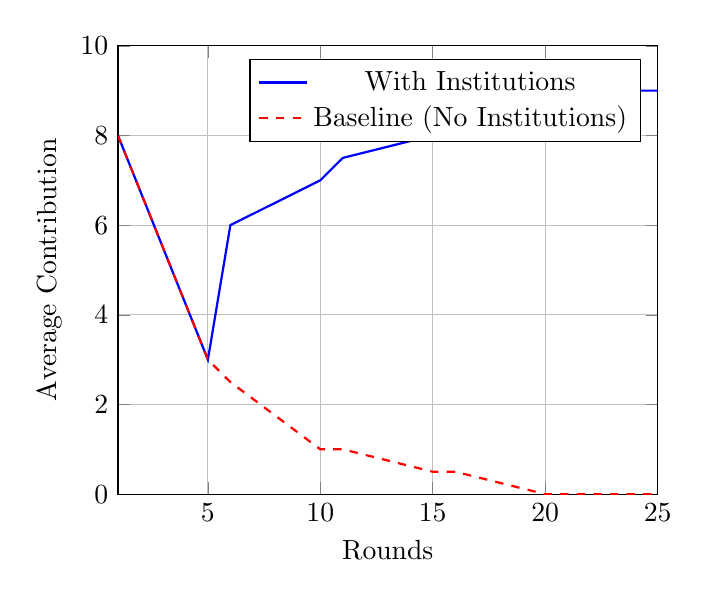
\begin{tikzpicture}
\begin{axis}[
    xlabel=Rounds,
    ylabel=Average Contribution,
    xmin=1, xmax=25,
    ymin=0, ymax=10,
    legend pos=north east,
    grid=both]
\addplot[blue, thick] coordinates {(1,8) (5,3) (6,6) (10,7) (11,7.5) (15,8) (16,8.5) (20,9) (21,9) (25,9)};
\addlegendentry{With Institutions}
\addplot[red, thick, dashed] coordinates {(1,8) (5,3) (6,2.5) (10,1) (11,1) (15,0.5) (16,0.5) (20,0) (21,0) (25,0)};
\addlegendentry{Baseline (No Institutions)}
\end{axis}
\end{tikzpicture}
\caption{Expected Contribution Trajectories}
\end{figure}

\subsection{Analysis Strategy}
\begin{enumerate}
\item \textbf{Descriptive Analysis}: Contribution patterns, voting frequencies, earnings distributions
\item \textbf{Hypothesis Testing}:
\begin{itemize}
\item H1: Logistic regression on first voting choice
\item H2: Mixed-effects models comparing efficiency across institutions
\item H3: Transition probability matrices and Markov chain analysis
\item H4: Learning models with experience-weighted attraction
\end{itemize}
\item \textbf{Efficiency Analysis}:
\begin{equation}
\text{Efficiency} = \frac{\text{Actual Total Earnings}}{\text{Maximum Possible Earnings}} \times 100\%
\end{equation}
\item \textbf{Path Dependence Tests}: 
\begin{equation}
P(\text{Retention}) = f(\text{Past Performance}, \text{Institution Type}, \text{Group Characteristics})
\end{equation}
\end{enumerate}

\section{Limitations and Possible Extentions}

\subsection{Limitations}
\begin{itemize}
\item Limited number of voting periods (4 elections)
\item Monetary stakes may not reflect real-world consequences
\item Potential order effects in institutional presentation
\end{itemize}

\subsection{Future Extensions}
\begin{itemize}
\item Different group sizes
\item Additional treatments with different starting points
\end{itemize}

\section{Conclusion}

This study provides a novel experimental framework for examining endogenous institutional choice in social dilemmas. By allowing groups to repeatedly select among multiple governance mechanisms, we capture the dynamic nature of institutional evolution that characterizes many real-world collective action problems. Our systematic comparison of individual vs. collective and punishment vs. reward mechanisms within a 2×2 framework advances beyond previous research that typically examines single institutions or imposed rules.

The findings will contribute to several literatures: experimental economics on institutional design, political economy on democratic decision-making, and organizational theory on self-governance. Practical applications include designing voting systems for environmental governance, corporate compliance mechanisms, and community resource management.
  
\bibliographystyle{chicago}
\bibliography{Literature}

\end{document}